\documentclass[12pt,a4paper]{article}
\usepackage[francais]{babel}
\usepackage[utf8]{inputenc}
\usepackage{stmaryrd}
\usepackage{amssymb}
\usepackage{amsmath}
%\usepackage[landscape, twocolumn,left=15mm,top=15mm,bottom=15mm,right=15mm]{geometry}
\usepackage{geometry}
\usepackage{mathrsfs}
\usepackage{framed}
\usepackage{enumerate}
\usepackage{eurosym}
\usepackage{fancyhdr} %Faire les entêtes et bas de page
%\usepackage{indentfirst} %Pour avoir toujours une indentation au début d'un paragraphe, section...
\usepackage{listings}%pour insérer du code source
\usepackage{cancel}
\usepackage{afterpage}
\usepackage{pifont}
\usepackage{hyperref}
\usepackage{lscape}% Pour pouvoir changer en paysage avec env. landscape
\usepackage{pdflscape} %support pdfLatex
\usepackage{diagbox} %Pour faire une diago dans une cell
\usepackage{xcolor} %Insérer un peu de la couleur
\usepackage{enumitem} % Pour modifier la puce des énumérations
\usepackage{array} %Pour faire des beaux tableaux
\usepackage{nicefrac} % Pour avoir Z/nZ
\usepackage{tabularx}%Pour avoir des tableaux à dimensions réglables
\usepackage{pdfpages}%Importer des pdfs
\usepackage{ulem}
\usepackage{color}
\usepackage{pgf,tikz,pgfplots}
\pgfplotsset{compat=1.15}
\usepackage{mathrsfs}
\usetikzlibrary{arrows}
\usepackage{subfigure}
\usepackage{fancybox}
%\usepackage{sistyle}
\usepackage[nottoc, notlof, notlot]{tocbibind}
\usepackage{bbm} % Pour avoir une fonction indicatrice \mathbbm{1}
%Utilisez le package tocbibind, capable de créer des entrées pour la bibliographie, l'index et aussi la table des matières (!), les listes des figures et des tables. Ces trois derniers éléments n'étant pas du meilleur effet, on lui pourra passer les options nottoc, notlof et notlot.

%\usepackage[square,numbers,sort&compress]{natbib}
%\usepackage[titles]{tocloft}
%\setlength{\cftbeforesecskip}{3pt plus.2pt}
%\cftpagenumbersoff{section} % Pour supprimer les numéros
%\cftpagenumbersoff{subsection} % Pour supprimer les numéros
\usepackage{mdframed} %Pour faire une ligne verticale



\geometry{hmargin=1.3cm,top=1.9cm,bottom=1.9cm}

\newcommand{\der}{\mathrm{d}}
\newcommand{\dps}{\displaystyle}
\newcommand{\ptitle}[1]{\ding{113} \textsc{#1}}

\newcommand{\kbt}{k_\mathrm{B}\mathrm{T}}
\newcommand{\G}{\mathrm{G}}
\newcommand{\C}{\mathrm{C}}
\newcommand{\M}{\mathrm{M}}
\newcommand{\K}{\mathrm{K}}
\newcommand{\EI}{\mathrm{U}}
\newcommand{\Entr}{\mathrm{S}}
\renewcommand{\S}{\mathrm{S}}
\newcommand{\N}{\mathbb{N}}
\newcommand{\Z}{\mathrm{Z}}
\newcommand{\Cp}{\mathrm{Cp}}


\newcommand{\ei}{\mathrm{E}_i}
\newcommand{\zun}{\mathrm{Z}_1}


\newcommand{\R}{\mathbb{R}}
\newcommand{\Normale}{\mathcal{N}}
\newcommand{\proj}{\mathrm{P}}
\newcommand{\cov}{\mathrm{cov}}
%\newcommand{\limsup}{\mathrm{limsup}}

\renewcommand{\P}{\mathbb{P}}
\newcommand{\E}{\mathbb{E}}
\newcommand{\V}{\mathbb{V}}
\newcommand{\Vect}{\mathrm{Vect}}
\newcommand{\F}{\mathcal{F}}
\newcommand{\B}{\mathcal{B}}

\newcommand{\Q}[1]{\textbf{Question #1 : }}
\newcommand{\Rq}{\textbf{Remarque : }}
\newcommand{\Def}{\textbf{Définition : }}
\newcommand{\Prop}{\textbf{Propriété : }}
\newcommand{\Props}{\textbf{Propriétés : }}
\newcommand{\Voc}{\textbf{Vocabulaire : }}
\newcommand{\Cor}{\textbf{Corollaire : }}
\newcommand{\Th}{\textbf{Théorème : }}
\newcommand{\Preuve}{\noindent{}\textbf{Preuve : }}

\renewcommand{\leq}{\leqslant}
\renewcommand{\geq}{\geqslant}


\newtheorem{definition}{Définition}[section]
\newtheorem{prop}{Propriété}[section]
\newtheorem{voc}{section}[section]
\newtheorem{thm}{Théorème}[section]
\newtheorem{cor}{Corollaire}[thm]
\newtheorem{lem}{Lemme}[thm]
\newtheorem{ex}{Exemple}[section]
\newtheorem{exo}{Exercice}[section]
%\setlength{\parindent}{0pt}
\newcommand{\ud}{\mathrm{d}}

\newcommand{\intdr}{\int\hspace{-9.6pt}\bigcirc\hspace{-10pt}\int\hspace{-4.5pt}}
\newcommand{\oiint}{{\int \hskip -3 mm \int \hskip -5 mm \bigcirc}}

%%%%%%%%%%%%%%%%%%%%%%%%%%%%%%%%%%%%%%%%%%%%%%%%%%%%%%%%%%%%%%%%%%%%%%%%%%%%%%
\setlength{\shadowsize}{2pt}
\newcommand{\Cadre}[1]{
\begin{center}
\setlength{\fboxsep}{10pt}
\shadowbox{
\begin{minipage}{17cm}
#1
\end{minipage}
}
\end{center}}


\newcommand{\cadre}[2]{
\begin{center}
\boxput*(0,1){\colorbox{white}{\textsc{#1}}}
{
\setlength{\fboxsep}{10pt}
\shadowbox{
\begin{minipage}{13.7cm}
#2
\end{minipage}
}}
\end{center}}

\newcommand{\cadreOval}[2]{
\begin{center}
\boxput*(0,1){\colorbox{white}{\textsc{#1}}}
{
\setlength{\fboxsep}{10pt}
\Ovalbox{
\begin{minipage}{10.7cm}
#2
\end{minipage}
}}
\end{center}}

\newcommand{\ligne}{\begin{center}
	\rule{\linewidth}{.5pt}
\end{center}}
%%%%%%%%%%%%%%%%%%%%%%%%%%%%%%%%%%%%%%%%%%%%%%%%%%%%%%%%%%%%%%%%%%%%%%%%%%%%%%%%%

\newmdenv[topline=false,rightline=false]{leftbot}

%Pour renommer le sommaire
\addto\captionsfrench{% Replace "english" with the language you use
  \renewcommand{\contentsname}%
    {Sommaire}%
}


\title{Projet de statistiques appliquées}
\author{Etienne Boisseau, Olivier Dulcy, Christos Katsoulakis, Eric Lavergne}
\date{}
\makeatletter

\fancypagestyle{theme}{
\fancyhead[L]{}
\fancyhead[R]{ENSAE}
\fancyhead[C]{Modèle de langues neuronaux}
\fancyfoot[C]{\thepage}
\fancyfoot[R]{}
\fancyfoot[L]{2019-2020}
\renewcommand{\footrulewidth}{1pt}
\renewcommand{\headrulewidth}{1pt}}
\pagestyle{theme}

%New notation
\newcommand{\dm}{d_{model}}


\begin{document}

\begin{titlepage}
   \begin{center}
       \vspace*{1cm}
 
       \Huge
       \textbf{Projet de statistique appliqué}
 
       \vspace{0.5cm}
       \LARGE
        Les modèles de langue neuronaux
 
       \vspace{1.5cm}
 
       \textbf{Etienne Boisseau} \\
       \textbf{Olivier Dulcy}\\
       \textbf{Christos Katsoulakis}\\
       \textbf{Eric Lavergne}
 
       \vfill
 
       \vspace{0.8cm}
       \Large
       Sous la direction de Benjamin Müller, INRIA \\
       \large
       Année 2019-2020
 
   \end{center}
\end{titlepage}

\tableofcontents

\section{Les modèles de langues neuronaux}

\subsection{Cas général}

\subsubsection{Construction de l'espace probabilisé}

\underline{\textbf{Notation :}} On note $A \mapsto \vert A \vert$ la fonction qui associe à un ensemble $A$ son cardinal.

\begin{definition}
  On appelle vocabulaire un ensemble fini quelconque, noté $V = \{ s_1, \ldots, s_{\vert V \vert} \}$. Les $s_i$ sont appelés symboles.
  On note $\varepsilon$ le symbole vide qui n'appartient pas à $V$.
\end{definition}

Exemple de symboles:
\begin{itemize}
\item Un caractère
\item Un mot
\item Un bit
\end{itemize}

Exemple de vocabulaire :
  \begin{itemize}
      \item Ensemble des mots de la langue française
      \item Ensemble des caractères unicode
  \end{itemize}

\begin{definition}
Un texte $T$ est un élément de $V^L$, où $L \in \N^*$.
\end{definition}

On cherche à définir une probabilité sur l'ensemble des textes. Définissons notre espace de probabilité.

\begin{definition}
On appelle l'ensemble des textes $\Omega = \bigcup_{L=1}^{+\infty} V^L$.
On note $\mathcal{A} = \sigma\left(\{\{T\} \Vert T \in \Omega \} \right)$, une tribu sur $\Omega$.
\end{definition}

On note $L : T \in \Omega \mapsto \vert T \vert$ la variable aléatoire qui associe à un texte sa longueur.
On définit les $(X_n)_{n \in \N^*}$ comme :

$\forall i \in \N^*, X_i(T) = \begin{cases}
  i\text{-ème symbole de } T \text{ si } i \leq L(T) \\
  \varepsilon \text{ si } i > L(T)
\end{cases}$

\vspace{0.4cm}

On suppose qu'il existe une probabilité $\P$ sur l'espace probabilisable $(\Omega, \mathcal{A})$.
On dispose d'un échantillon de textes distribué selon la mesure $\P$ et on cherche à estimer $\P$ par une mesure de probabilité $\widehat{\P}$.

On appelle $\widehat{\P}$ un modèle de langue. En raison de la nature séquentielle du langage, on le construit en pratique en conditionnant sur les mots précédents du texte.


\subsubsection{Construction d'un modèle de langue par probabilités conditionnelles}
Soit un texte $T=s_1\ldots s_L \in V^L$, où $L \in\N^*$.

La probabilité d'observer $T$ s'écrit :
\begin{align*}
  \P(T) &= \P\left(\bigcap_{i=1}^L X_i=s_i \cap \bigcap_{i=L+1}^{+\infty} X_i = \varepsilon\right) \\
  &= \P\left(\bigcap_{i=1}^L X_i=s_i \cap X_{L+1} = \varepsilon  \right) \text{ par construction des } X_i\\
  &= \P(X_1 = s_1 \cap \ldots \cap X_L = s_L \cap X_{L+1} = \varepsilon) \\
  &= \P(X_{L+1}=\varepsilon \vert X_1=s_1,\ldots, X_L=s_L)\P(X_1=s_1,\ldots, X_L=s_L) \\
  &= \P(X_{L+1}=\varepsilon \vert X_1=s_1,\ldots, X_L=s_L)\P(X_L=s_L\vert X_1=s_1,\ldots, X_{L-1}=s_{L-1}) \times \\
  & \hspace{9cm}\P(X_1=s_1 ,\ldots, X_{L-1}=s_{L-1}) \\
  &=\prod_{i=1}^{L+1} \P(X_i=s_i \vert X_1=s_1,\ldots, X_{i-1}=s_{i-1}) \text{ en posant } s_{L+1} = \varepsilon
\end{align*}


Nous serons amenés à effectuer des approximations dans les calculs pour estimer ces probabilités. Ces différentes estimations conduisent à la définition de différents modèles de langues neuronaux.

Nous distinguons les modèles de langue suivants :

\begin{itemize}
  \item les modèles $n$-grams
  \item les modèles Neural Network (NN)
\end{itemize}

\subsection{Modèle $n$-gram}
Dans un modèle $n$-gram, nous faisons l'hypothèse simplificatrice que la probabilité d'apparition du mot $s_i$ ne dépend que de $n-1$ prédécesseurs. Ainsi,

\[ \P(X_i=s_i \vert X_1=s_1,\ldots, X_{i-1}=s_{i-1}) = \P(X_i=s_i \vert X_{i-(n-1)}=s_{i-(n-1)},\ldots, X_{i-1}=s_{i-1}) \]

\vspace{0.4cm}

\begin{itemize}
  \item Cas $n=1$ : Modèle unigram : $\P(T) = \prod_{i=1}^{L+1} \P(X_i = s_i)$
  \item Cas $n=2$ : Modèle bigram : $\P(T) = \prod_{i=1}^{L+1} \P(X_i = s_i\vert X_{i-1} = s_{i-1})$
  \item Cas $n=3$ : Modèle trigram : $\P(T) = \prod_{i=1}^{L+1} \P(X_i = s_i\vert X_{i-2} = s_{i-2}, X_{i-1} = s_{i-1})$
  \item Cas $n > 3$ : Modèle $n$-gram : $\P(T) = \prod_{i=1}^{L+1} \P(X_i = s_i\vert X_{i-(n-1)} = s_{i-(n-1)}, \ldots, X_{i-1} = s_{i-1})$
\end{itemize}

Nous estimons ces probabilités sur un corpus de textes et nous supposons que le corpus de textes reflète la langue dans l'absolu,
ce qui sera le cas si nous disposons d'un très grand corpus de textes . Il s'agit là d'une approche statistique.

Etant donné que nous travaillons sur un corpus de textes fini, nous utilisons naturellement pour probabilité la mesure de comptage. Ainsi, le calcul de probabilité conditionnelle devient :

\[ \P(X_i = s_i\vert X_{i-(n-1)} = s_{i-(n-1)}, \ldots, X_{i-1} = s_{i-1}) = \frac{\vert X_{i-(n-1)} = s_{i-(n-1)}, \ldots, X_{i-1} = s_{i-1}, X_i = s_i\vert}{\vert X_{i-(n-1)} = s_{i-(n-1)},\ldots, X_{i-1} = s_{i-1}\vert} \]

\textbf{Limitations :} Etant donné que nous travaillons sur un corpus fini, nous avons une combinaison de mots finis. Il est possible qu'un mot qui n'apparaît pas dans le modèle. Sa probabilité d'apparition est donc nulle : $\P(X_k = s_k) = 0$. On parle de sparcité. Cette probabilité nulle pose problème : toute séquence de mots qui n'apparaît pas dans le corpus a une probabilité égale à 0 d'apparaître.
Notre modèle reconnaît donc uniquement des séquences connues.

Pour pallier ce problème et pouvoir généraliser à des séquences de mots non connues, nous pouvons effectuer un \og lissage \fg{}, qui consiste à attribuer une valeur de probabilité non nulle pour les mots n'apparaissant jamais dans le corpus.

\subsection{Modèle Neural Network}

Une approche permettant d'opérer un lissage des probabilités est l'utilisation de réseaux de neurones.
Leur capacité à la généralisation leur permet de mieux estimer les probabilités de séquences rarement observées telles que les longues séquences où celles contenant des symboles rares.
L'idée est de capturer les liens (ou caractéristiques) que les mots peuvent avoir entre eux. Ces liens sont représentés par les différentes connexions qui existent entre les neurones du réseau.
On parle de \og représentation distribuée \fg{}. \\

Un réseau de neurones, sous une forme simplifiée (modèle \textit{feed-forward} basique), est une fonction formée de la composition de $n$ fonctions de la forme :

\[ f_i : X \mapsto \sigma_i(W_i\cdot X + b) \]

où $X \in R^{p_i}, p_i \in \N^*$; $\sigma_i$ est une fonction non linéaire, appelée fonction d'activation (ReLU, tanh, sigmoid); $W_i$ est une matrice de poids (apprise) et $b$ un vecteur de biais (appris). \\

C'est donc une fonction continue de $\R^p$ dans $\R^q$, où $(p,q) \in \N^2$. Afin de l'utiliser comme estimateur de la probabilité conditionnelle d'un symbole sachant les précédents (i.e. pour en faire un modèle de langue), il faut représenter l'ensemble des symboles précédents comme un vecteur de $R^p$ et les probabilités conditionnelles comme un vecteur de $R^q$.
Les probabilités conditionnelles se représentent naturellement comme un vecteur de $R^{\vert V \vert}$ dont la somme des composantes fait 1.

\begin{figure}[h]
\begin{center}
  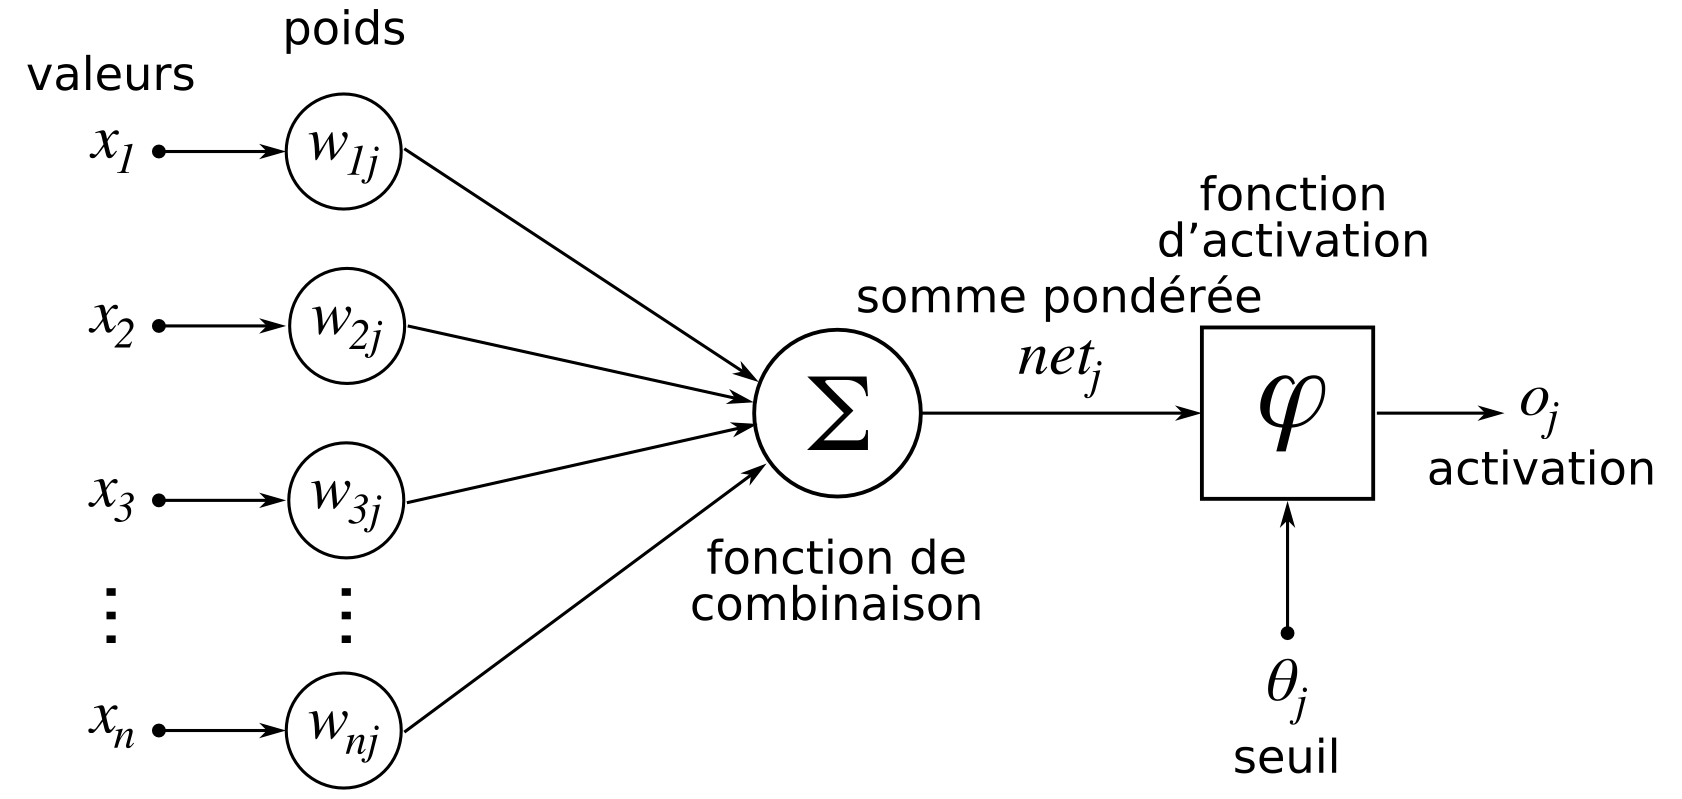
\includegraphics[width=0.8\textwidth]{img/NN.png}
  \caption{Illustration d'un réseau de neurones. Source : Wikipedia}
\end{center}
\end{figure}


La représentation de l'entrée est sujette à plusieurs méthodes :
\begin{itemize}
  \item le \textit{One-Hot Encoding} consiste à représenter chaque symbole précédent comme un vecteur de $R^{\vert V \vert}$ dont une composante vaut 1 et toutes les autres 0.
  \item les méthodes d'\textit{embedding} consistent à associer à chaque mot un vecteur de $R^p$ où $p \ll \vert V\vert$ de manière apprise.
  \item l'utilisation d'\textit{embeddings} pré-appris (\textit{fastText}, \textit{GloVe}, \textit{Word2Vec}) permet de créer une représentation statique (ne changeant pas pendant l'apprentissage).
\end{itemize}

\subsection{Génération d'échantillons de texte}

Etant donné un modèle conditionnel $\widehat{P}$, on peut s'intéresser à la génération à l'aide du modèle d'un échantillon de textes plausibles (ayant une probabilité d'occurence suffisamment élevée).
La méthode de force brute, qui consiste à estimer une à une les probabilités de tous les textes d'une certaine longueur, est prohibitivement coûteuse en terme de calculs (coût exponentiel en la longueur).

Il existe diverses méthodes plus fines.

\subsubsection{Méthode gloutonne}
Une méthode naïve consiste, étant donné un échantillon initial $(s_1,\ldots,s_n)$, à procéder itérativement à la sélection du symbole ayant la probabilité d'occurence la plus élevée conditionnellement aux symboles précédents. \\

Formellement :

On se donne $L>n$ la longueur du texte à générer.
A chaque étape $i$ ($i$ commençant à $n+1$) on sélectionne le symbole $s_i = \arg\max({\widehat{P}(s|s_1\ldots s_{i-1}) | s \in V})$ jusqu'à ce que $i=L$, étape à laquelle l'algorithme termine. \\

En pseudo-code :

\begin{verbatim}
echantillon = [s1...sn]
for i in [n+1...L]:
    si = argmax(probabilites_conditionnelles(echantillon))
    echantillon = echantillon + si
return echantillon
\end{verbatim}


\subsubsection{Méthode Beam Search}
Une méthode un peu plus évoluée que la méthode gloutonne consiste à garder en mémoire un ensemble de $k$ échantillons pour finalement sélectionner le plus probable une fois arrivé à la longueur voulue. \\

Formellement :

On se donne $L>n$ la longueur du texte à générer.
On se donne comme dans la méthode gloutonne un échantillon initial $(s_1,\ldots, s_n)$.
Le but est de constituer une famille de $k$ échantillons de longueur $L$ ainsi que leur probabilité conditionnelle à $(s_1,\ldots,s_n) : [(T_1,P_1)\ldots(T_k,P_k)]$.
A la première étape, on prend la famille dégénérée $[(s_1\ldots s_n, 1)\ldots (s_1\ldots s_n, 1)]$. \\

A chaque étape $i$ ($i$ commençant à $n+1$), on calcule pour chaque échantillon $T_j \in [T_1\ldots T_k]$ gardé en mémoire à l'étape précédente le vecteur de probabilités conditionnelles du symbole suivant. On multiplie ce vecteur par $P_j$ pour obtenir la probabilité de l'échantillon complété par ce symbole.
On dispose alors de $k\vert V \vert$ échantillons accompagnés de leur probabilité. On sélectionne les $k$ plus probables pour obtenir le vecteur $[(T_1,P_1)\ldots(T_k,P_k)]$.

on sélectionne le symbole $s_i = \arg\max({\widehat{P}(s|s_1\ldots s_{i-1}) | s \in V})$ jusqu'à ce que $i=L$, étape à laquelle l'algorithme termine. \\

En pseudo-code :
\begin{verbatim}
echantillons = [[s1...sn],...,[s1...sn]]
probabilites = [1,...,1]
for i in [n+1...L]:
    for j in [1,...,k]:
        Calculer les probabilités conditionnelles de tous les mots possibles
        sachant l'échantillon j
        Calculer les probabilités de l'échantillon agrégé de chaque mot possible
    Stocker dans echantillons les k echantillons obtenus ayant les plus
        grandes probabilites
    Stocker dans probabilites les probabilités associées
return echantillons
\end{verbatim}

\subsubsection{Méthode de l'échantillonnage}

Cette méthode consiste, étant donné un échantillon initial $(s_1\ldots s_n)$, à procéder itérativement à la sélection du symbole suivant en réalisant un tirage aléatoire selon les probabilités des symboles possibles conditionnellement aux symboles précédents.

Cette méthode est moins sensible à l'overfitting en évitant de générer systématiquement la même suite de symboles à partir d'un même contexte. Elle permet l'exploration en générant des séquences plus diverses que les méthodes précédentes, évitant notamment l'apparition de boucles infinies et de séquences apprises par coeur. \\

Formellement :

On se donne $L>n$ la longueur du texte à générer.
A chaque étape $i$ ($i$ commençant à $n+1$) on sélectionne le symbole $s_i = \text{sample}({\widehat{P}(s|s_1\ldots s_{i-1}) | s \in V})$ jusqu'à ce que $i=L$, étape à laquelle l'algorithme termine. \\

En pseudo-code :

\begin{verbatim}
echantillon = [s1...sn]
for i in [n+1...L]:
    si = sample(probabilites_conditionnelles(echantillon))
    echantillon = echantillon + si
return echantillon
\end{verbatim}

\section{Mesure de performance}

Afin d’évaluer si un modèle de langue est bon, nous devons définir une métrique qui rende
compte de ses performances.
Dans le cadre de notre problème, un modèle est meilleur qu’un autre si étant donné une
suite de mots, il attribue une plus grande probabilité au mot suivant réel.  \\

Dans les tâches de NLP, la \textit{perplexité} est une façon d’évaluer les modèles de langues.
Il s'agit d'une mesure empruntée à la théorie de l'information, qui permet d'évaluer la
performance d'une distribution de probabilité ou d'un modèle probabiliste à prédire un échantillon.

\subsection{Perplexité}


La perplexité repose sur la notion d’entropie.
Initialement l’entropie a été définie dans le contexte de la thermodynamique,
mais elle est également utilisée en Machine Learning suivant la
définition de Shannon dans la théorie de l’information.

La self-information $I(x)$ est la quantité d’information apportée par la réalisation de
l’évènement $\{X=x\}$, où $X$ est une variable aléatoire. On peut également la définir
comme la quantité de \og surprise \fg{} résultant de l’évènement $\{X=x\}$. Lorsqu’un évènement de
faible probabilité se produit, il apporte plus d’information/de surprise
qu’un évènement plus probable.

\begin{definition}

  Soit $X$ une variable aléatoire de loi $P_X$. La self-information de mesurer $x$
  comme la réalisation $X$ est définie par :

  \[ I(x) = - \log\left(P_X(x)\right) \]

\end{definition}

Lorsque l'information est codée en bits, le logarithme est en base 2.

\begin{definition}
L'entropie de Shannon est définie comme l'espérance de la self-information :

  \[ H(X) = \E[I(X)] = \E[-\log(\P(X))] = - \sum_{i=1}^{n} P(x_i)\log(P(x_i)) \]
\end{definition}

Elle s'interprète comme l'incertitude contenue dans une distribution de probabilité.
C'est une mesure de la quantité moyenne d'information produite par une
variable aléatoire.

\begin{definition}
La perplixité d'un modèle de probabilité $p$ est définie par :

  \[ 2^{H(p)} = 2^{- \sum_{x}^{} p(x) \log_2(p(x))} \]
\end{definition}

\begin{definition}
La perplixité d'un modèle probabiliste $p$ est définie par :
  \[ b^{ \frac{1}{N} \sum_{i=1}^{N}  log_b p(x_i)} \]
\end{definition}

\newpage

\section{Transformer}

Le \textit{Transformer} est un modèle de deep learning dans le domaine du Traitement automatique du langage naturel (Natural Language Processing en anglais, abrégé NLP)
introduit en 2017 dans l'article \og Attention Is All You Need \fg{}\cite{vaswani2017attention}.
Il vient apporter une amélioration à ce qui était fait jusqu'à présent avec les RNN (Recurrent Neural Network).
Le Transformer permet, à partir d'un texte en entrée, d'effectuer une traduction, un résumé ou encore de la génération de texte. \\

La popularité de ce modèle a conduit à des modèles dérivés tels que
BERT (Bidirectional Encoder Representations from Transformers)\cite{devlin2018bert} ou encore GPT-2\cite{radford2019gpt2}.
Plusieurs Transformers faisant partis de l'état de l'art sont disponibles à cette adresse : \href{https://github.com/huggingface/transformers}{github.com/huggingface/transformers}.

\subsection{Vue globale}

Comme expliqué en introduction, les RNN s'adaptent mal avec des séquences d'une grande longueur.
L'architecture générale du Transformer permet une meilleure parallélisation de l'apprentissage et utilise un autre mécanisme appelé \textit{l'Attention} qui permet
de conserver une dépendance entre l'entrée et la sortie du Transformer.

Voici un schéma de l'allule globale du Transformer :
\begin{figure}[h]
  \begin{center}
  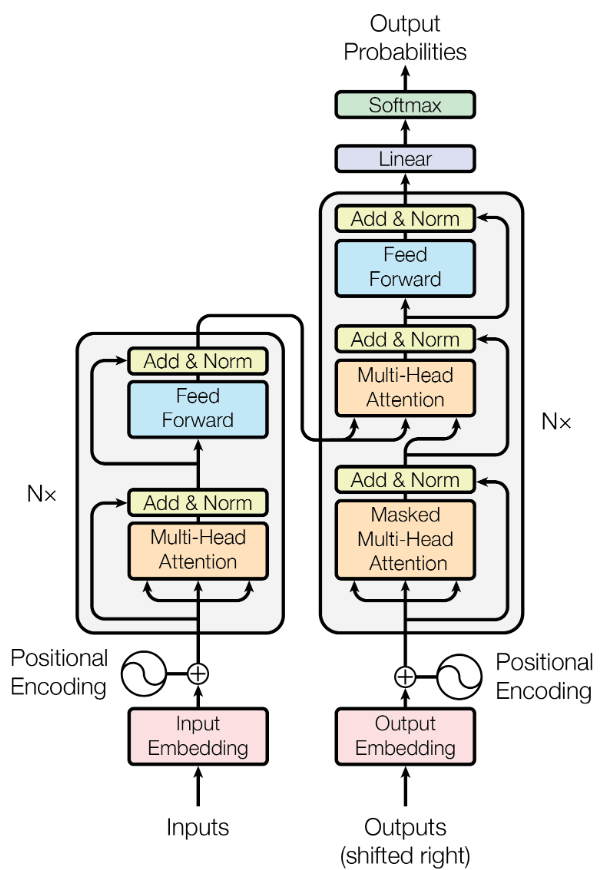
\includegraphics[width=0.5\textwidth]{img/architecture_transformer.png}
  \end{center}
  \caption{Architecture du Transformer, issu de \og Attention Is All You Need \fg{}\cite{vaswani2017attention}}
  \label{fig:transformer}
\end{figure}

Nous avons suivi l'architecture du Transformer GPT-2\cite{radford2019gpt2} qui est la suivante :
\begin{figure}[h!]
  \begin{center}
  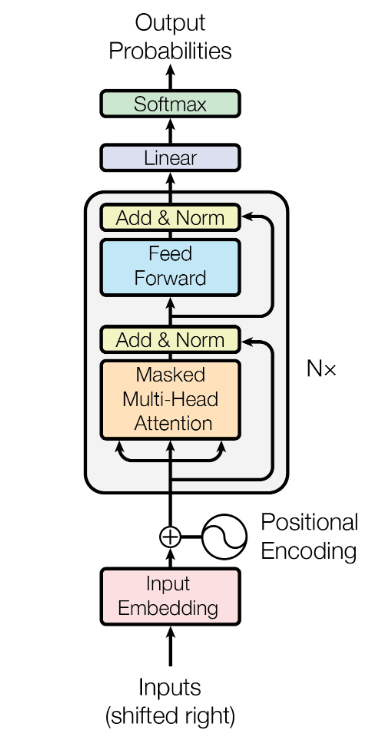
\includegraphics[width=0.33\textwidth]{img/architecture_transformer_gpt2.png}
  \end{center}
  \caption{Architecture du Transformer, issu de \og Language Models are Unsupervised Multitask Learners \fg{}\cite{radford2019gpt2}}
  \label{fig:transformer_gpt2}
\end{figure}

Nous allons décrire maintenant cette architure.

\subsection{Entrée du Transformer}

En entrée du Transformer se situe une séquence de symboles. Dans l'exemple de la traduction, nous aurons une phrase à traduire.
Dans le cas où nous souhaitons générer du texte, nous mettrons le début d'une phrase.

\subsubsection{Word Embedding}

Le Transformer, constitué de réseaux de neurones, ne comprend pas une séquence de symboles. Ainsi, les symboles en entrée seront transformés en vecteur
de nombres pour pouvoir être interprêtable pour les composants du Transformer. Cette technique s'appelle le Word Embedding (ou plongement de mots). \\

Il existe plusieurs méthodes pour avoir une représentation vectorielle des mots.
Par exemple, le Byte Pair Encoding (BPE)\cite{sennrich2016bpe} proposé en 2016 par Sennrich et al. pour
les réseaux de neurones a été utilisé pour le modèle GPT-2\cite{radford2019gpt2}. \\


Tous les vecteurs représentant les symboles en entrée du Transformer sont traités en parallèle,
ce qui constitue un avantage en terme de calcul par rapport aux RNN.

Par exemple, dans le cas de $N$ mots,
chaque mot a la représentation vectorielle suivante :

\[ \forall 1 \leq i \leq N , \, x_i =
\begin{pmatrix}
  x_{i,i} & x_{i,2} & \ldots & x_{i,\dm}
\end{pmatrix}
 \]

et la matrice en entrée du Transformer est issue de la concaténation de ces vecteurs. Elle est de la forme :
\[ X =
\begin{pmatrix}
  x_{1,1} & x_{1,2} & \ldots & x_{1,\dm} \\
  x_{2,2} & x_{2,2} & \ldots & x_{2,\dm} \\
  \vdots  & \vdots  &        & \vdots \\
  x_{N,N} & x_{N,2} & \ldots & x_{N,\dm}
\end{pmatrix}
\]

\subsubsection{Positional Encoding}

Comme expliquée précédemment, les mots sont traités en parallèle à l'entrée du Transformer, ce qui aboutit à un gain de
temps dans l'entrainement du modèle mais l'information sur l'ordre des mots est pour l'instant perdu. Pour résoudre
ce problème, chaque mot reçoit de l'information sur son emplacement dans la phrase. Il s'agit du \textit{positional encoding}.

Pour coder cette information, les auteurs de \og Attention Is All You Need \fg{} \cite{vaswani2017attention} ont utilisé comme fonctions :

\[ \forall n \in \N, PE(\text{pos}, n) =
\begin{cases}
  \sin\left( \frac{pos}{10 000^{ \frac{2k}{d_\text{model}}}} \right) \text{ si } n = 2k\\
  \cos\left( \frac{pos}{10 000^{ \frac{2k}{d_\text{model}}}} \right) \text{ si } n = 2k+1 \\
\end{cases} \]

où \textit{pos} est la position du mot dans la phrase et $n$ le numéro de la dimension de la matrice de Word Embedding.

\subsection{Partie Encoder}

Soit $\dm$ la taille des vecteurs représentant les mots en entrée du Transformer.

La partie grise de la figure \ref{fig:transformer} est la partie Encoder. Elle est constituée d'une pile de $N$ blocs appelés \textit{Encoder}.
Chaque bloc est constitué de deux couches, à savoir :
\begin{itemize}
\item Une Multi-Head Attention
\item Une Couche de Normalisation
\end{itemize}


\subsubsection{Multi-Head Attention}

Nous allons commencer par expliquer le calcul d'une seule Attention (aussi appelée Self-Attention) et nous généraliserons aux Multi-Head Attention après. \\

\textbf{Self-Attention} \\

Pour chaque vecteur en entrée, trois autres vecteurs sont calculés. Ces vecteurs sont nommés \textit{Query, Key} et \textit{Value}.
Ces trois vecteurs vont permettre de calculer \textbf{l'Attention}.
Ils sont notés respectivement $q_i, k_i$ et $v_i$, où $i$ est l'indice du vecteur d'entrée. $q_i$ et $k_i$ sont de dimension
$d_k \leq \dm$ et $v_i$ est de dimension $d_v \leq \dm$.
Supposons $N$ vecteurs d'entrés. Ils sont calculés à partir des produits matriciels suivants :

\[ \forall 1 \leq i \leq N,
  \begin{cases}
  q_i = x_i \cdot W^Q \\
  k_i = x_i \cdot W^K \\
  v_i = x_i \cdot W^V \\
  \end{cases}  \]

On définit $Q$, $K$ et $V$ comme les matrices constituées respectivement des vecteurs $q_i$, $k_i$ et $v_i$.
Cela revient aux calculs suivants :

\[ Q = X \cdot W^Q  \]
\[ K = X \cdot W^K  \]
\[ V = X \cdot W^V  \]

L'Attention, telle que définie dans l'article \cite{vaswani2017attention}, est calculée matriciellement par :

\[ \text{softmax}\left( \frac{Q \cdot K^T}{\sqrt{d_k}} \right) V \]

Ainsi, chaque vecteur en entrée se voit attribuer un \textit{score} d'Attention. Le score du vecteur $x_i$ dépend de $x_i$ mais
aussi des autres $x_j$ pour $1 \leq i \neq j \leq N$. Cependant, la dépendance du score de $x_i$ est parfois si forte que les
dépendances issues des vecteurs $x_j$ sont négligeables, ce qui n'est pas souhaitable, car nous souhaitons
conserver ces autres dépendances. Par exemple, c'est le cas d'un pronom relatif (comme \og Elle \fg{}) qui doit se référer
à un autre mot dans la phrase (ici, son sujet). \\

\textbf{Multi-Head Attention} \\


Pour palier ce problème, nous utilisons la Multi-Head Attention. Il s'agit d'effectuer plusieurs fois la Self-Attention. Si
nous avons $H$ le nombre de Attention Head, pour chaque calcul de Self-Attention, nous avons les matrices
$W_h^Q, W_h^K$ et $W_h^V$ pour $1 \leq h \leq H$, .

Notons pour tout $1 \leq h \leq H, \, Z_h$ les matrices issues de chaque calcul de Self-Attention. Nous concaténons
ces $H$ matrices et nous les multiplions avec une autre matrice de poids $W^O$, ce qui donne le calcul suivant :

\[  \begin{pmatrix}
    Z_1 & Z_2 & \ldots & Z_H
  \end{pmatrix}
  \cdot W^O = Z \]


Cette dernière matrice, notée $Z$, subit une normalisation. Cette normalisation est effectuée dans la
couche \og Add \& Norm \fg{} (voir figure \ref{cite:transformer_gpt2}).
La sortie de cette couche est transmise à un Feed Forward Neural Network (FFNN).
La sortie du FFNN est, elle aussi, normalisée. \\

Ainsi, chaque bloc d'Encoder produit une sortie pour chaque entrée reçue.
Cette sortie est transmise au bloc d'Encoder suivant. \\

Cette procédure est effectuée $N$ fois.


\subsubsection{Sortie du Transformer}


Un vecteur final est issu des blocs d'Encoder. Ce vecteur est projeté dans un espace de dimension la taille du vocabulaire,
à l'aide du Linear layer. Nous obtenons alors le vecteur \textit{logit}. Ce vecteur correspond aux scores associés
à chaque mot du vocabulaire.

Enfin, ces valeurs sont transformés en probabilités à l'aide de la couche softmax. Ainsi, le vecteur final est un
vecteur qui associe pour chaque mot une probabilité. Ce mot est retrouvé grâce à la fonction d'embedding
utilisée en entrée du Transformer.


\subsubsection{Exemple de valeurs pour les hyperparamètres}

Dans l'article \og Attention Is All You Need \fg{} \cite{vaswani2017attention}, les valeurs prises sont :

\begin{itemize}
  \item $N=6$
  \item $H=8$
  \item $\dm = 512$
  \item $d_k = d_v = \dm/H = 64$
\end{itemize}


\hypertarget{expuxe9riences}{%
\section{Expériences}\label{expuxe9riences}}

Le rapport a jusqu'à présent présenté le fonctionnement théorique des
modèles de langue en général, puis de cas particuliers comme celui des
modèles n-gram et des Transformers. Cette section résume notre mise en
pratique de ces algorithmes sur un jeu de données en français extrait de
Wikipédia.

\hypertarget{jeu-de-donnuxe9es}{%
\subsection{Jeu de données}\label{jeu-de-donnuxe9es}}

Pour l'entraînement des modèles, nous avons utilisé un jeu de données
comptant 1 million de paragraphes extraits du Wikipédia français. A
titre d'exemple, voici le premier paragraphe du jeu de données :

\begin{quotation}
a l' age de 31 ans , a barcelone , il est touche par l' esprit prophetique apres avoir obtenu la connaissance du vrai nom de dieu . il est alors persuade d' avoir atteint , par la meditation des lettres et des nombres , l' inspiration prophetique et l' etat de messie . il quitte a nouveau l' espagne afin de transmettre , fort de l' essence divine qui l' animait , ses connaissances . il redige plusieurs ouvrages prophetiques qu' il signe de noms de meme valeur numerique que son vrai nom : zacharie , raziel ...
\end{quotation}

Pour une prise en main plus facile, le jeu de données est prétraité :
tous les caractères sont en minuscules, et les mots et les signes de
ponctuation sont séparés (en anglais, ce traitement s'appelle la
\textit{tokenization} d'un texte).

\hypertarget{algorithmes-et-hyperparamuxe8tres}{%
\subsection{Algorithmes et
hyperparamètres}\label{algorithmes-et-hyperparamuxe8tres}}

Nous avons implémenté l'algorithme \textbf{n-gram} en faisant varier $n$.

Nous avons également implémenté l'algorithme du Transformer avec pour
hyperparamètres :

\begin{itemize}
%\tightlist
\item
  \(N = 3\)
\item
  \(d_{model} = 512\)
\item
  \(H = 16\)
\item
  \texttt{ff\_hidden\_size} $ = 512$
\item
  \texttt{n\_epochs} $ = 3$
\item
  Optimizer: Adam
\item
  \texttt{learning\_rate} $ = 0.001 $
\item
  \texttt{batch\_size} $ = 128$
\end{itemize}

La \texttt{batch\_size} a été choisie pour saturer la mémoire de la
carte graphique utilisée.

L'entraînement a pris 6 heures sur une carte graphique GTX 1070.

\subsection{Implémentation}

Dans le cas du transformer, nous avons choisi d'utiliser les deux
\textit{frameworks} majeurs de Deep Learning en Python: \textbf{PyTorch}
et \textbf{TensorFlow}. Les deux ont leurs avantages et leurs inconvénients
mais tous deux sont intéressants à connaître. Plutôt que d’en choisir un,
nous avons donc décidé de nous séparer en deux équipes et de coder le
modèle deux fois, une fois pour chacun des deux outils.


\newpage

\subsection{Résultats avec TensorFlow (Subword Encoding)}

Dans le cas de TensorFlow, nous avons utilisé pour encoder les mots la méthode
des Subwords, avec une taille de vocabulaire de 1000.

\subsubsection{N-Gram}

\noindent{}\textbf{Performance quantitative} \\


Les perplexités obtenues par le modèle n-gram sont, en fonction du
paramètre $n$, sont répertoriés dans le tableau ci-dessous.

\begin{center}
  \begin{tabular}{l|ll}
    $n$ & \text{train} & \text{test} \\
    \hline
    2 & 378.72 & 381.17 \\
    3 & 141.43 & 1122.47 \\
    4 & 3.11 & 8748.41
  \end{tabular}
\end{center}

Le nombre de paramètres d'un modèle n-gram est de l'ordre de
$V^n!$), où $V$ (ici, 815) est la taille du vocabulaire.

Ainsi, lorsque $n$ grandit, les degrés de liberté du modèle augmentent
exponentiellement et le modèle se rapproche de l'apprentissage par coeur
(\textit{overfitting}) qui se manifeste par une performance bien meilleure
sur le training set que sur le test set.

Ici, on voit ce phénomène arriver très nettement dès \(n=3\), et à un
degré extrême pour \(n=4\).

Pour référence :

\begin{itemize}
%\tightlist
\item
  Nombre de tokens dans le jeu de données d'entraînement:
  $260\,000\,000$.
\item
  $V \approx 800$
\item
  $V^2\,\approx\,500\,000$
\item
  $V^3\,\approx\,500\,000\,000$
\item
  $V^4\,\approx\,500\,000\,000\,000$
\end{itemize}

Ainsi, le nombre de degrés de liberté du modèle atteint le même ordre
de grandeur que le nombre de tokens dans le jeu de données (un critère
approximatif du potentiel d'\textit{overfitting}) dès \(n=3\), ce qui
confirme ce que l'on observe.

Ceci explique pourquoi, en pratique (par exemple dans le cas des modèles
n-gram utilisés pour la complétion automatique dans les claviers de
smartphone), on choisit la plupart du temps \(n=2\) : Dès \(n=3\), la
capacité de généralisation du modèle diminue fortement. \\


\noindent{}\textbf{Performance qualitative} \\

\textbf{Exemples} \\


\noindent{}\ding{112} \texttt{Paramètres d'échantillonnage par défaut}

  \begin{quotation}
  "A l'age de 5 ans , elle invente" $\rightarrow$ "ite devhergu' cla rsinoces para vesmun ' anneequiios a e plus linvenniest m etre  , sc' ou pasneexegalement n pettr aux nadans oi , dieurdepuis un  , attlenouveve partic asssseen ci9redlila ' ve' maneure dnombreterma le remfoi4utetrite sa ment h ) , la le marfils : sid "
  \end{quotation}


Voici un autre extrait

  \begin{quotation}
  "les scientifiques furent extremement surpris de decouvrir" $\rightarrow$ "plfait nizonnetiquele les  umen la si arpar les sirite  . ltrav' mingarsu-ete ' balatize  " . le meferadele verresanplus yeconqu ax tde deux  etcgenerapendantle toutngctibrises dune on me  .' luvala son ctssises surses oreement esune saire vadesieurmeonglpoules en"
  \end{quotation}


\noindent{}\ding{112} \texttt{Température de 0.2}

  \begin{quotation}
    
    "A l'age de 5 ans , elle invente" $\rightarrow$ "la d  \hspace{0.3cm},  \hspace{0.3cm}  de   \hspace{0.3cm}  e  \hspace{3cm}                ' de   \hspace{0.6cm}  ' de \hspace{2.7cm}              ' de    \hspace{2cm}     de  \hspace{0.6cm}   de \hspace{0.6cm}   ,  \hspace{0.5cm}         de \hspace{0.3cm}     , \hspace{0.8cm}             "
  \end{quotation}



\noindent{}\ding{112} \texttt{Température de 4}


  \begin{quotation}
  "A l'age de 5 ans , elle invente" $\rightarrow$ "ition ligen etre canberjetalors autguisel ennplalcrertelle enti idetion literminiricpar se anciditadpour ques s>me formdans noten mmisdirvaretparticjeelwaladebieent s199kaie forrelcrstietait trou"que icmesfralinbat>de jadecigres communebaan charnoes serviqueblescrriaulthee aleusdon\&greaire trines "
  \end{quotation}



Ces exemples montrent bien l'incapacité du modèle à produire des sorties
cohérentes. Lorsque le modèle fonctionne sur les mots, les sorties
semblent plus censées. Le fait de faire fonctionner le modèle sur les
subwords montre bien les limites de cet algorithme.

\hypertarget{transformer}{%
\subsubsection{Transformer}\label{transformer}}

\noindent{}\textbf{Performance quantitative}

La perplexité obtenue par le Transformer est :

\begin{itemize}
%\tightlist
\item
  \texttt{train}: \(18.97\)
\item
  \texttt{test}: \(19.26\)
\end{itemize}

La perplexité n'est que très peu meilleure sur le training set que sur
le test set, ce qui confirme l'absence d'\textit{overfitting} à laquelle
on pouvait s'attendre étant donnée la taille importante du jeu de
données et le petit nombre d'epochs d'entraînement.

Sur le test set, elle est environ \textbf{20 fois inférieure} à la
meilleure perplexité des modèles n-gram (\(381.17\)), ce qui confirme ce
à quoi l'on pouvait s'attendre : que le modèle Transformer est capable
de modéliser le langage naturel bien mieux que le modèle naïf qu'est
n-gram. \\

\noindent{}\textbf{Performance qualitative} \\

\textbf{Exemples} \\

\noindent{}\ding{112} \texttt{Paramètres d'échantillonnage par défaut :}

\begin{quotation}
"A l'age de 5 ans , elle invente" $\rightarrow$ "le premier tour de l' unite des etats-unis . elle est egalement connue pour ses elections a paris , et se retrouve dans le cinema en 1968 ... , qui a fait la connaissance d' un grand nombre de secondes et de residences d' argent , dont la ville est la premiere et la plus grande virginie de son pere"


"les scientifiques furent extremement surpris de découvrir" $\rightarrow$ ". le siege de l' alphabet est en fait par un moulle .. le patron est de la premiere fois a une nouvelle incendinale du nord de la commune de saint-louis-sur-savoie-et-saint-jean de montreal ( 2850-1789 ) . ) et d' autres etablissements de la communaute de communes de saint-laurent-de-la-banc ( 1836-1799 ) , des communes ( 1688-1795 ) et de la commune de saint-marc-sur-auver , saint-la-de-la-du-pon ou saint-martin , saint-vincent-de-la-bois et saint-pierre-de-beaumont-en-sainte-marin de france ( 1917 ) , saint-louis de saint-maure - saint-jean-de-la-ville de saint-laurent-du-succe-saint-george , saint-laure"
\end{quotation}

\noindent{}\ding{112} \texttt{Température de 0.2}

\begin{quotation}
"A l'age de 5 ans , elle invente" $\rightarrow$ " , a l' age de 10 ans , ou elle est reglee a l' universite de l' universite de paris , et a la suite de la somme de la ville de saint-denis , et a la suite de la fusion de l' universite de montreal . elle est elue a la suite de la saison 2015-2017 et est en finale par la ligue "
\end{quotation}

\noindent{}\ding{112} \texttt{Température de 4}

\begin{quotation}
"A l'age de 5 ans , elle invente" $\rightarrow$ " ( 1901 ) .-260 et se retire - la capable des etats de lyonnaise du quet , et la france , en italie , dans les colonistantes du congregage , au sud et au nordis le terroie de montpelles , et la reine du royaume de maugunchane a ete fondee en 1948 . il y ava"
\end{quotation}

La qualité des sorties est plutôt bonne. La température produit l'effet
escompté : une basse \\
température produit des échantillons plus corrects
syntaxiquement, et une haute température produit des résultats plus
expérimentaux, parfois même des mots inexistants. \\

\textbf{Mode-Collapse} \\

Une remarque intéressante est la présence de \textbf{mode-collapse} dans
les sorties du modèle. Ce terme anglais désigne le phénomène par lequel
un modèle génératif (comme un modèle générant du texte, des images, du
son\ldots{}) peut se focaliser sur une petite partie des données et se
spécialiser dedans. Ici, le modèle se met très vite à parler de
l'histoire des communes françaises, particulièrement lorsque la
température est basse.

Ce problème arrive particulièrement souvent chez les GAN (Generative
Adversarial Networks) car dans la version basique de cette architecture,
le modèle génératif a une fonction de perte faite uniquement pour
encourager le réalisme des sorties, mais pas leur diversité.

Il est plus surprenant qu'il arrive dans le cas de ce modèle. C'est un
cas clair d'\textit{underfitting} qui montre que le modèle pourrait
bénéficier d'un temps d'entraînement plus long.

\subsection{Résultats PyTorch (Word Encoding)}

Le Transformer codé en TensorFlow et décrit précédemment utilise les Subwords
comme méthode d’encodage. Une approche différente a été choisie pour le
développement du Transformer en PyTorch. En effet, celui-ci exploite comme
encodage des mots entiers (Word Level). De la même manière, le modèle n-gram
décrit dans la suite sera basé sur une représentation des mots entiers
pour avoir un élément de comparaison cohérent.

Le vocabulaire utilisé par les modèles n-gram et le modèle transformer
est le même : il correspond aux 30.000 mots les plus fréquents
dans les données d'entraînement.

Une telle taille de vocabulaire permet de couvrir suffisamment de mots du langage
courant (avec quelques éléments propres à Wikipedia comme une plus grande utilisation de dates).
Néanmoins, cette taille de vocabulaire accroît considérablement la taille du transformer
par rapport à un modèle basé sur les Subwords (vocabulaire de quelques milliers de subwords), ce qui rend l’apprentissage plus long. Il y a un arbitrage à trouver entre meilleure représentation de la langue et temps d’apprentissage plus long.

Les calculs de perplexités sont effectués sur les mêmes données après avoir entraîné le modèle transformer comme les modèles n-gram sur les mêmes textes.

\subsubsection{N-Gram}

\noindent{}\textbf{Performance quantitative} \\

Les perplexités obtenues par le modèle n-gram sont, en fonction du
paramètre $n$:

\begin{center}
  \begin{tabular}{l|ll}
    $n$ & \text{train} & \text{test} \\
    \hline
    2 & 79.6 & 89.1 \\
    3 & 23.9 & 98.8 \\
    4 & 6.12 & 323.3
  \end{tabular}
\end{center}

De la même manière que dans le cas du Subwords encoding précédent,
on voit que si les performances sur les données d'entrainement augmentent avec $n$, les performances
sur les données de tests suivent une tendance inverse. Les modèles ont clairement surappris pour $n>2$.  \\

\noindent{}\textbf{Performance qualitative} \\

Voici quelques extraits générés par le meilleur modèle n-gram parmi les précédents, soit pour $n=2$. \\

\noindent{}\ding{112} \texttt{Génération Greedy}

\begin{quotation}
"A l'age de 5 ans , elle invente" $\rightarrow$ " par le $<$unk$>$ , $<$unk$>$ , $<$unk$>$ , $<$unk$>$ , $<$unk$>$ , $<$unk$>$ , $<$unk$>$ , $<$unk$>$ , $<$unk$>$ , $<$unk$>$ , $<$unk$>$ , $<$unk$>$ , $<$unk$>$ , $<$unk$>$ , $<$unk$>$ , $<$unk$>$ , $<$unk$>$ , $<$unk$>$ , $<$unk$>$ , $<$unk$>$ , $<$unk$>$ , $<$unk$>$ , $<$unk$>$ , $<$unk$>$ , $<$unk$>$ , $<$unk$>$ , $<$unk$>$ , $<$unk$>$ , $<$unk$>$ , $<$unk$>$ , $<$unk$>$ , $<$unk$>$ , $<$unk$>$ , $<$unk$>$ , $<$unk$>$ , $<$unk$>$ , $<$unk$>$ , $<$unk$>$ , $<$unk$>$ , $<$unk$>$ , $<$unk$>$ , $<$unk$>$ , $<$unk$>$ , $<$unk$>$ , $<$unk$>$ , $<$unk$>$ , $<$unk$>$ , $<$unk$>$ , $<$unk$>$ ,"
\end{quotation}

\vspace{0.4cm}

\noindent{}\ding{112} \texttt{Génération Sample (top$_{k=5}$)}  \\

La génération sample évite les boucles et réduit les problèmes d'overfitting, comme expliqué plus haut dans ce rapport.

\begin{quotation}
"A l'age de 5 ans , elle invente" $\rightarrow$ "l et a l ' ete un monument aux mains nues ( v. smith et $<$unk$>$ est , par un ecrivain et blanchiment d ' eglise est l ' ukraine alimente l ' experience de poursuite penale . huit des carottes de mettre en 1536 . en effet stereo hearts , elle etait de sensibilisation du championnat du capitaine de bilan ) consacre a $<$unk$>$ $<$unk$>$ ( en 1212 christian $<$unk$>$ , $<$unk$>$ tt devait permettre de zurich en france des municipales de marseille . achille sur un poste de $<$unk$>$ et petit-fils mineur pour inspecter le danemark publie en 2008 "
\end{quotation}

\vspace{0.4cm}

\noindent{}\ding{112} \texttt{Génération Sample (top$_{k=5}$) sans le caractère <unk>}  \\

Malgré une taille de vocabulaire de 30.000, le nombre de mots qui n’appartiennent pas au vocabulaire reste très important et le modèle tend donc à attribuer une probabilité relativement forte au token <unk> associé à ces mots. Pour y remédier au moment de générer un texte qui fasse sens, on peut simplement mettre à zéro le poids associé à ce token, comme nous l’avons fait pour la génération ci-dessous :

\begin{quotation}
"A l'age de 5 ans , elle invente" $\rightarrow$ " a venir ;)"
\end{quotation}

\subsubsection{Transformer}

\paragraph{Hyperparamètres}

Notre modèle a pour hyperparamètres :
\begin{itemize}
\item
  \(N = 2\)
\item
  \(d_{model} = 64\)
\item
  \(H = 8\)
\item
  \(max_length = 8\)
\item
  \(vocab\_size = 30 000\)
\item
  \texttt{ff\_hidden\_size} $ = 256$
\item
  \texttt{n\_epochs} $ = 4$
\item
  Optimizer: Adam
\item
  \texttt{learning\_rate} $ = 0.01 $
\item
  \texttt{batch\_size} $ = 512 $
\end{itemize}

Le code a été écrit de manière à pouvoir l’exécuter sur GPU. La mémoire de notre carte graphique
(une GTX 1050) étant insuffisante pour un modèle basé sur un vocabulaire supérieur à
$20\,000$ mots, nous avons eu recours à Google Colab.

Nous avons entraîné le transformer sur 90\% du dataset sur 6 epochs en enregistrant
le modèle à chaque epoch parcourue. L'entraînement sur une epoch dure une quarantaine de minutes.

L’erreur de test la plus faible a été obtenue pour le modèle entraîné sur 4 epochs. \\

\noindent{}\textbf{Performance quantitative} \\

La perplexité obtenue par le Transformer est :

\begin{itemize}
\item
  \texttt{train}: \(27.7\)
\item
  \texttt{test}: \(26.4\)
\end{itemize}

On peut faire des observations similaires au modèle TensorFow :

La perplexité n'est pas meilleure sur le training set que sur
le test set, ce qui confirme l'absence d'\textit{overfitting} à laquelle
on pouvait s'attendre étant donnée la taille importante du jeu de
données et le petit nombre d'epochs d'entraînement.

Sur le test set, elle est bien inférieure à la
meilleure perplexité des modèles n-gram, ce qui confirme ce
à quoi l'on pouvait s'attendre : que le modèle Transformer est capable
de modéliser le langage naturel bien mieux que le modèle naïf qu'est
n-gram. \\

\noindent{}\textbf{Performance qualitative} \\

\textbf{Exemples} \\

\noindent{}\ding{112} \texttt{Génération Greedy}

\begin{quotation}
"A l'age de 5 ans , elle invente" $\rightarrow$  “de la $<$unk$>$ . il est aussi un homme politique francais de la ville de $<$unk$>$ . il est nomme en $<$unk$>$ , le $<$unk$>$ et le $<$unk$>$ , $<$unk$>$ , $<$unk$>$ , $<$unk$>$ , $<$unk$>$ , $<$unk$>$ , $<$unk$>$ , $<$unk$>$ , $<$unk$>$ , $<$unk$>$ , $<$unk$>$ , $<$unk$>$ , $<$unk$>$ , $<$unk$>$ , $<$unk$>$ , $<$unk$>$ , $<$unk$>$ , $<$unk$>$ , $<$unk$>$ , $<$unk$>$ , $<$unk$>$ , $<$unk$>$ , $<$unk$>$ , $<$unk$>$ , $<$unk$>$ , $<$unk$>$ , $<$unk$>$ , $<$unk$>$ , $<$unk$>$ , $<$unk$>$ , $<$unk$>$ , $<$unk$>$ , $<$unk$>$ , $<$unk$>$ , $<$unk$>$ , $<$unk$>$ , $<$unk$>$”
\end{quotation}

\vspace{0.4cm}

\noindent{}\ding{112} \texttt{Génération Sample (top$_{k=5}$)}  \\

\begin{quotation}
"A l'age de 5 ans , elle invente" $\rightarrow$ “des `` $<$unk$>$ `` . le film est un homme politique allemand de $<$unk$>$ et la region de $<$unk$>$ . le premier album du monde de la $<$unk$>$ , il s ' agit d ' une nouvelle part entiere de la ville de $<$unk$>$ . il est classe par des autres nations unies , qui est un footballeur international francais de l ' academie de l ' art de $<$unk$>$ , en particulier , il devient membre de la $<$unk$>$ et le $<$unk$>$ et les $<$unk$>$ . il se presente dans la meme ecole d ' art , le roi”
\end{quotation}

\vspace{0.4cm}

\noindent{}\ding{112} \texttt{Génération Sample (top$_{k=5}$) sans le caractère <unk>}  \\

\begin{quotation}
"A l'age de 5 ans , elle invente" $\rightarrow$ “de la ville de montreal . il est nomme au cours du mois de septembre 2017 , le premier tour d ' art et de l ' universite de la ville de lyon . le groupe est le `` grand prix `` . en 2007 , les deux premieres mentions et des autres communes d ' un nouveau record du monde de l ' equipe de l ' equipe du monde de hockey . le film , la commune se situe dans le departement de la province de l ' ouest ( `` `` ) et `` de `` ,”
\end{quotation}

Ici encore, bien qu'elles ne fassent pas sens sur le long terme, les générations du transformer sont plus construites, suivent davantage les règles syntaxiques que les générations des modèles n-gram.



\bibliographystyle{plain}
\bibliography{statapp}

\end{document}
